% general format definition
\documentclass[a4paper, 11pt]{article}
\usepackage[margin=.9in]{geometry}
\usepackage[utf8]{inputenc}
\usepackage[T1]{fontenc}
\usepackage[english]{babel}

% extra packages
\usepackage{hyperref}
\usepackage{listings}
\usepackage{color}
\usepackage{amssymb}
\usepackage{amsmath}
\usepackage{mathtools}
\usepackage{microtype}
\usepackage{stmaryrd}
\usepackage{tikz}
\usepackage{booktabs}
\usepackage{stmaryrd}
\usepackage{enumitem}
\usepackage{multirow}


% special math symbols
\newcommand{\R}{\ensuremath{\mathbb{R}}}
\newcommand{\N}{\ensuremath{\mathbb{N}}}
\newcommand{\Z}{\ensuremath{\mathbb{Z}}}
\newcommand{\Q}{\ensuremath{\mathbb{Q}}}

% logical operators
\newcommand{\xor}{\ensuremath{\oplus}} %exklusives oder
\newcommand{\impl}{\ensuremath{\rightarrow}} %logische Implikation

% nicer symbols
\renewcommand{\phi}{\varphi}
\renewcommand{\theta}{\vartheta}
\renewcommand{\epsilon}{\varepsilon}

% Syntax highlighting
\definecolor{commentsColor}{rgb}{0.497495, 0.497587, 0.497464}
\definecolor{keywordsColor}{rgb}{0.000000, 0.000000, 0.635294}
\definecolor{stringColor}{rgb}{0.558215, 0.000000, 0.135316}
\definecolor{brightlavender}{rgb}{0.75, 0.58, 0.89}
\definecolor{brilliantrose}{rgb}{1.0, 0.33, 0.64}
\definecolor{canaryyellow}{rgb}{1.0, 0.94, 0.0}
\definecolor{cyan}{rgb}{0.0, 1.0, 1.0}
\definecolor{fulvous}{rgb}{0.86, 0.52, 0.0}
\definecolor{olive}{rgb}{0.5, 0.5, 0.0}
\lstset{
  backgroundcolor=\color{white},                        % choose the background color; you must add \usepackage{color} or \usepackage{xcolor}
  basicstyle=\footnotesize,                             % the size of the fonts that are used for the code
  breakatwhitespace=false,                              % sets if automatic breaks should only happen at whitespace
  breaklines=true,                                      % sets automatic line breaking
  captionpos=b,                                         % sets the caption-position to bottom
  commentstyle=\color{commentsColor}\textit,            % comment style
  deletekeywords={},                                    % if you want to delete keywords from the given language
  escapeinside={\%*}{*)},                               % if you want to add LaTeX within your code
  extendedchars=true,                                   % lets you use non-ASCII characters; for 8-bits encodings only, does not work with UTF-8
  frame=tb,	                   	                        % adds a frame around the code
  keepspaces=true,                                      % keeps spaces in text, useful for keeping indentation of code (possibly needs columns=flexible)
  keywordstyle=\color{keywordsColor}\bfseries,          % keyword style
  otherkeywords={True,False,true,false,null,None,NULL}, % if you want to add more keywords to the set
  numbers=left,                                         % where to put the line-numbers; possible values are (none, left, right)
  numbersep=5pt,                                        % how far the line-numbers are from the code
  numberstyle=\tiny\color{commentsColor},               % the style that is used for the line-numbers
  rulecolor=\color{black},                              % if not set, the frame-color may be changed on line-breaks within not-black text (e.g. comments (green here))
  showspaces=false,                                     % show spaces everywhere adding particular underscores; it overrides 'showstringspaces'
  showstringspaces=false,                               % underline spaces within strings only
  showtabs=false,                                       % show tabs within strings adding particular underscores
  stepnumber=1,                                         % the step between two line-numbers. If it's 1, each line will be numbered
  stringstyle=\color{stringColor},                      % string literal style
  tabsize=2,	                                          % sets default tabsize to 2 spaces
  title=\lstname,                                       % show the filename of files included with \lstinputlisting; also try caption instead of title
  columns=fixed,                                        % Using fixed column width (for e.g. nice alignment)
}

\author{Thilo Metzlaff\\406247 \and Mats Frenk\\393702\and Emma van Emelen\\406008}
\title{BUS Exercise 8 \\ Group 23}
\begin{document}
    % titlepage
    \maketitle
    \newpage

    % contents
    \tableofcontents
    \newpage

    % section 0
    \section*{Introduction}
    And again i have the wonderful task of doing this. Somehow i wasted way too much time again. 

    \subsection*{THE FORMAT}
    \begin{itemize}
      \item Every file will be named similar to the sections in here, so\\
      \texttt{2.1-stack\_exercise.c} is Exercise 2, section 1.
      \item Every Solution \textbf{WILL} be in this pdf, but not necessarily 
            anything predefined by the exercise.
      \item Anysegmentxtbf{WARNING:} Humor may or may not be used. If you are allergic
            to humor, that sounds like a personal problem.
      \item \textbf{WARNING:} Backing up your data is important. Although linux 
            doesn't have the necessary shame to remove itself, unlike windows\footnote{Happened to me... too often},
            please do back up your data. And try to keep track of your periods\dots
            they seem to be notoriously hard to find
    \end{itemize}
    \newpage
    
    \section{Memory management}
    \subsection{Shared memory}
    Let's say we request a memory block of length n. in this case, we get a pointer to that address which also has the data about its own length. Now, let's say this block is fragmented, then we get a page file. 
    This pake file would then hold the amount of blocks needed as well as their exact locations in memory. Since we work with memory pointers, and the pointers must point to the exact same place, they should logically use the same page file.
    Otherwise we would populate our memory with a bunch of duplicate data, which would be inefficient in both time (memory access latency) and space. Therefore the processes probably use the same logical addresses.
    
    \subsection{Page Marking}
    If pages have to be swapped, we can see which page has meen modified. This way we don't have to check for changes, but rather we can see if something has been modified and then reload without checking the whole data set.

    \subsection{Copy-on-Write}
    This saves on processing time, since the child only gets things from daddy, if it tries to write to that block of memory.

    \subsection{Error handling?}
    This would only need more processing time with only a marginal improvement, since the Algorithms tend to be more complicated and are more about making educated guesses, than the errors are.
    Error handling of this kind should only be implemented if it is truly critical that everything is absolutely correct . 
    \newpage
    \section{Demand Paging}
    \subsection{Paging Strategies}
    \setlength{\tabcolsep}{3.5mm}
      \renewcommand{\arraystretch}{1.2}
      \begin{center}
      \begin{tabular}{|r||r|r|r|r|r|r|r|r|r|r|r|r|r|r|r|}
      \multicolumn{16}{l}{\textbf{Strategy: FIFO}}\\
      \hline
            Referenz $\omega$ & 0 & 1 & 2 & 3 & 2 & 4 & 5 & 2 & 6 & 3 & 4 & 7 & 8 & 7 & 8 \\
      \hline\hline
            Frame 1    & 0  & 0  &0   & 0  & 0  & 4  & 4  &  4 & 4  & 4  & 4  & 4  & 8  & 8  & 8  \\\hline
            Frame 2    &    &  1 &  1 &  1 & 1  & 1  & 5  &  5 & 5  &5   & 5  & 5  & 5  & 5  & 5  \\\hline
            Frame 3    &    &    &  2 &  2 & 2  & 2  & 2  & 2  & 6  & 6  & 6  & 6  & 6  & 6  & 6  \\\hline
            Frame 4    &    &    &    &  3 &  3 & 3  & 3  & 3  & 3  & 3  & 3  & 7  & 7  & 7  & 7  \\
      \hline\hline
            Priority 1 & 0  & 1  & 2  & 3  & 3  & 4  & 5  & 5  & 6  & 6  & 6  & 7  & 8  & 8  & 8  \\\hline
            Priority 2 &    & 0  & 1  & 2  & 2  &  3 & 4  & 4  & 5  & 5  & 5  & 6  & 7  & 7  & 7  \\\hline
            Priority 3 &    &    & 0  & 1  & 1  & 2  & 3  & 3  & 4  & 4  & 4  & 5  & 6  & 6  & 6  \\\hline
            Priority 4 &    &    &    & 0  & 0  & 1  &2   &2   & 3  & 3  & 3  & 4  & 5  & 5  & 5  \\
      \hline\hline
            Paging Error  & x  & x  & x  & x  &   & x  & x  &   & x  &   &   & x  & x  &   &   \\
      \hline
      \multicolumn{16}{l}{\textbf{Paging Errors: 9}}\\
      \end{tabular}
      \end{center}

      \vfill

      \begin{center}
      \begin{tabular}{|r||r|r|r|r|r|r|r|r|r|r|r|r|r|r|r|}
            \multicolumn{16}{l}{\textbf{Strategie: LRU}}\\
            \hline
                  Reference $\omega$ & 0 & 1 & 2 & 3 & 2 & 4 & 5 & 2 & 6 & 3 & 4 & 7 & 8 & 7 & 8 \\
            \hline\hline
                  Frame 1    &0&0&0&0&0&4&4&4&4&3&3&3&3&3&3   \\\hline
                  Frame 2    &&1&1&1&1&1&5&5&5&5&4&4&4&4&4   \\\hline
                  Frame 3    &&&2&2&2&2&2&2&2&2&2&7&7&7&7   \\\hline
                  Frame 4    &&&&0&0&1&3&3&4&5&2&6&3&3&3   \\
            \hline\hline
                  Priority 1 &0&1&2&3&2&4&5&2&6&3&4&7&8&7&8   \\\hline
                  Priority 2 &&0&1&2&3&2&4&5&2&6&3&4&7&8&7   \\\hline
                  Priority 3 &&&0&1&1&3&2&4&5&2&6&3&4&4&4   \\\hline
                  Priority 4 &&&&0&0&1&3&3&4&5&2&6&3&3&3   \\
            \hline\hline
                  Paging Error  &x&x&x&x&&x&x&&x&x&x&x&x&&   \\
            \hline
            \multicolumn{16}{l}{\textbf{Paging Errors: 11}}\\
      \end{tabular}
      \end{center}


      \begin{center}
      \begin{tabular}{|r||r|r|r|r|r|r|r|r|r|r|r|r|r|r|r|}
            \multicolumn{16}{l}{\textbf{Strategy: SC}}\\
            \hline
                  Reference $\omega$ & 0 & 1 & 2 & 3 & 2 & 4 & 5 & 2 & 6 & 3 & 4 & 7 & 8 & 7 & 8 \\
            \hline\hline
                  Frame 1    &0&0&0&0&0&4&4&4&4&3&3&3&3&3&3   \\\hline
                  Frame 2    &&1&1&1&1&1&5&5&5&5&4&4&4&4&4   \\\hline
                  Frame 3    &&&2&2&2&2&2&2&2&2&2&7&7&7&7   \\\hline
                  Frame 4    &&&&3&3&3&3&3&6&6&6&6&8&8&8   \\
            \hline\hline
                  Priority 1 &0&1&2&3&3&4&5&5&6&3&4&7&8&8&8   \\\hline
                  Priority 2 &&0&1&2&2&3&4&4&2&6&3&4&7&7&7   \\\hline
                  Priority 3 &&&0&1&1&2&3&3&5&2&6&3&4&4&4   \\\hline
                  Priority 4 &&&&0&0&1&2&2&4&5&2&6&3&3&3   \\
            \hline\hline
                  Paging Error  &x&x&x&x&&x&x&&x&x&x&x&x&&   \\
            \hline
            \multicolumn{16}{l}{\textbf{Paging Errors: 11}}\\
      \end{tabular}
      \end{center}

      \begin{center}
      \begin{tabular}{|r||r|r|r|r|r|r|r|r|r|r|r|r|r|r|r|}
            \multicolumn{16}{l}{\textbf{Strategy: LFU}}\\
            \hline
                  Reference $\omega$ & 0 & 1 & 2 & 3 & 2 & 4 & 5 & 2 & 6 & 3 & 4 & 7 & 8 & 7 & 8 \\
            \hline\hline
                  Frame 1    &0&0&0&0&0&4&4&4&4&3&3&3&8&8&8   \\\hline
                  Frame 2    &&1&1&1&1&1&5&5&5&5&4&4&4&4&4   \\\hline
                  Frame 3    &&&2&2&2&2&2&2&2&2&2&2&2&2&2   \\\hline
                  Frame 4    &&&&3&3&3&3&3&6&6&6&7&7&7&7   \\
            \hline\hline
                  Priority 1 &0&1&2&3&3&4&5&5&6&3&4&7&8&8&8   \\\hline
                  Priority 2 &&0&1&2&2&3&4&4&5&6&3&4&7&7&7   \\\hline
                  Priority 3 &&&0&1&1&2&3&3&4&5&6&3&4&4&4   \\\hline
                  Priority 4 &&&&0&0&1&2&2&2&2&2&2&2&2&2   \\
            \hline\hline
                  Paging Error  &x&x&x&x&&x&x&&x&x&x&x&x&&   \\
            \hline
            \multicolumn{16}{l}{\textbf{Paging Errors: 11}}\\
      \end{tabular}
      \end{center}

      \begin{center}
      \begin{tabular}{|r||r|r|r|r|r|r|r|r|r|r|r|r|r|r|r|}
            \multicolumn{16}{l}{\textbf{Strategy: CLIMB}}\\
            \hline
                  Reference $\omega$ & 0 & 1 & 2 & 3 & 2 & 4 & 5 & 2 & 6 & 3 & 4 & 7 & 8 & 7 & 8 \\
            \hline\hline
                  Frame 1    &0&0&0&0&0&0&0&0&0&0&0&0&0&0&0   \\\hline
                  Frame 2    &&1&1&1&1&1&1&1&1&1&1&1&1&1&1   \\\hline
                  Frame 3    &&&2&2&2&2&2&2&2&2&2&2&2&2&2   \\\hline
                  Frame 4    &&&&3&3&4&5&5&6&3&4&7&8&7&8   \\
            \hline\hline
                  Priority 1 &0&0&0&0&0&0&0&2&2&2&2&2&2&2&2   \\\hline
                  Priority 2 &&1&1&1&2&2&2&0&0&0&0&0&0&0&0   \\\hline
                  Priority 3 &&&2&2&1&1&1&1&1&1&1&1&1&1&1   \\\hline
                  Priority 4 &&&&3&3&4&5&5&6&3&4&7&8&7&8   \\
            \hline\hline
                  Paging Error  &x&x&x&x&&x&x&&x&x&x&x&x&x&x   \\
            \hline
            \multicolumn{16}{l}{\textbf{Paging Errors: 13}}\\
      \end{tabular}
      \end{center}
      \begin{center}
      \begin{tabular}{|r||r|r|r|r|r|r|r|r|r|r|r|r|r|r|r|}
            \multicolumn{16}{l}{\textbf{Strategy:}}\\
            \hline
                  Reference $\omega$ & 0 & 1 & 2 & 3 & 2 & 4 & 5 & 2 & 6 & 3 & 4 & 7 & 8 & 7 & 8 \\
            \hline\hline
                  Frame 1    &0&0&0&0&0&4&4&4&4&4&4&4&8&8&8   \\\hline
                  Frame 2    &&1&1&1&1&1&5&5&5&5&5&5&5&5&5   \\\hline
                  Frame 3    &&&2&2&2&2&2&2&6&6&6&6&6&6&6   \\\hline
                  Frame 4    &&&&3&3&3&3&3&3&3&3&7&7&7&7   \\
            \hline\hline
                  Priority 1 &0&1&2&2&2&2&2&3&3&4&6&7&7&8&8   \\\hline
                  Priority 2 &&0&1&3&3&3&3&4&4&6&5&6&8&7&7   \\\hline
                  Priority 3 &&&0&1&1&4&4&5&6&5&4&5&6&6&6   \\\hline
                  Priority 4 &&&&0&0&1&5&2&5&3&3&4&5&5&5   \\
            \hline\hline
                  Paging Error  &x&x&x&x&&x&x&&x&&&x&x&&   \\
            \hline
            \multicolumn{16}{l}{\textbf{Paging Errors: 9}}\\
      \end{tabular}
      \end{center}
      \newpage
      \subsection[What if it's too big?]{What if it's too big?\footnote{then it don't fit, duh}}
      If the time interval is too big, then a page may be given a higher priority due to a higher perceived usage at the start (more time must be better), which then makes the page be held in memory unnecessarily, even if it isn't used.

      \section[Who's Better? - The ultimate comparison.]{Who's Better? - The ultimate comparison.\footnote{Spoiler: length doesn't matter}}
      \subsection{what if we fail? Who do we kill?}
      \subsubsection{Fifi's BFF}
      Page 2, since that one came first\footnote{at least that's what she said}.
      \subsubsection{LRU}
      Page 4, since we didn't access this for the longest amount of time
      \subsubsection{What we all deserve.}
      Page 3, since this is the oldest page with $A_3=1$
      \subsubsection{NRU}
      Page 0, since $D_0=0 \mbox{ } \land \mbox{ } A_0=0$

      \subsection{can we CLIMB to the top?}
      We cannot say with certainty which page is loaded next, since we would have to know how often the page was accessed. 
      We can however say, that Page 2 is guaranteed to not be loaded, since $A_2=1$and this page must be punished for coming first.
      Page 3 is a decent candidate for being swapped, since it was loaded later, giving it a low priority and $A_3=0$, 
      therefore nothing accessed this page a,d the priority didn't have a chance to get higher.
      \newpage
      \section{Lifetime function}
      \subsection{Paging errors and the value of life}
      \begin{center}
      \begin{tabular}{|r||r|r|}
            \hline
            $m$ & PF & $L(m)$\\\hline\hline
            1 & 17 & 1.18\\\hline
            2 & 16 & 1.25\\\hline
            3 & 13 & 1.54\\\hline
            4 & 7  & 2.86\\\hline
            5 & 7  & 2.86\\\hline
            6 & 6  & 3.33\\\hline
            7 & 6  & 3.33\\\hline
            8 & 6  & 3.33\\\hline
      \end{tabular}
      \end{center}
            
      \subsection{the Function of life}
      \begin{center}
      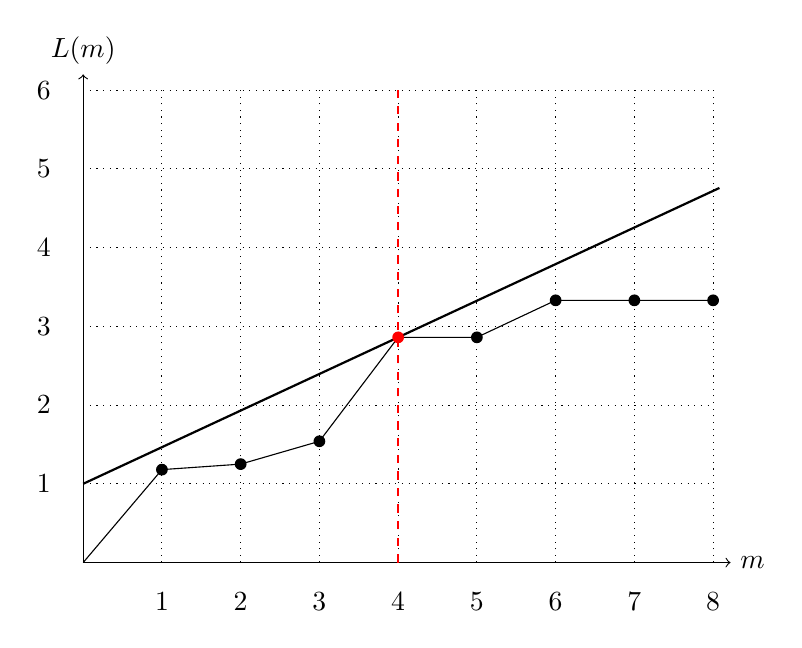
\begin{tikzpicture}
            \def\xsize{8}
            \def\ysize{6}
            \draw[thin, dotted] (0,0) grid (\xsize,\ysize);
            \foreach \x in {1,2,...,\xsize}
            \node at (\x, -0.5) {$\x$};
            \foreach \y in {1,2,...,\ysize}
            \node at (-0.5, \y) {$\y$};
            
            \node (xlabel) at (\xsize + 0.5,0) {$m$};
            \draw[->] (0,0) -- (xlabel);
            \node (ylabel) at (0,\ysize + 0.5) {$L(m)$};
            \draw[->] (0,0) -- (ylabel);

            % Beispiel Gerade durch Punkt:
            \draw[] (0,0) -- (1,1.18) -- (2,1.25) -- (3,1.54) -- (4,2.86) -- (5,2.86) -- (6,3.33) -- (8,3.33);
            \draw[thick,shorten >=-4.5cm] (0,1) -- (4,2.86);
            \draw[dashed,thick, color=red] (4,0) -- (4,6);


            % Beispiel Punkt:
            %\node at (2,3)[circle,fill,inner sep=1.5pt]{};
            
            \node at (1,1.18)[circle,fill,inner sep=1.5pt]{};
            \node at (2,1.25)[circle,fill,inner sep=1.5pt]{};
            \node at (3,1.54)[circle,fill,inner sep=1.5pt]{};
            \node at (4,2.86)[circle,fill,inner sep=1.5pt, color=red]{};
            \node at (5,2.86)[circle,fill,inner sep=1.5pt]{};
            \node at (6,3.33)[circle,fill,inner sep=1.5pt]{};
            \node at (7,3.33)[circle,fill,inner sep=1.5pt]{};
            \node at (8,3.33)[circle,fill,inner sep=1.5pt]{};

            

      \end{tikzpicture}
      \end{center}
      The Optimal frame would be 4, as defined by the ominous sounding knee-criterion. 
      \\What does it do? where will it go? we will kneever know...

\end{document}